\documentclass[11pt,a4paper,oneside]{report}
\usepackage[T1]{fontenc}
\usepackage[utf8]{inputenc}
\usepackage{charter}
\usepackage[scaled=0.86]{helvet}
\renewcommand{\ttdefault}{lmtt}
\usepackage{microtype}
\usepackage[a4paper,top=2.6cm,bottom=2.6cm,left=2.8cm,right=2.6cm,headheight=14pt]{geometry}
\usepackage{setspace}
\setstretch{1.18}
\usepackage[dvipsnames,table]{xcolor}
\definecolor{ink}{HTML}{0F172A}
\definecolor{accent}{HTML}{1F5FAD}
\definecolor{amberx}{HTML}{B45309}
\definecolor{rosex}{HTML}{BE123C}
\definecolor{okgreen}{HTML}{047857}
\definecolor{muted}{HTML}{475569}
\definecolor{soft}{HTML}{F1F5F9}
\usepackage{graphicx}
\usepackage{booktabs}
\usepackage{tabularx}
\usepackage{longtable}
\usepackage{array}
\usepackage{multirow}
\usepackage{enumitem}
\setlist{itemsep=2pt,topsep=4pt}
\usepackage{caption}
\captionsetup{font={small,sf},labelfont={bf,color=accent},labelsep=period,justification=raggedright,singlelinecheck=false}
\usepackage[most]{tcolorbox}
\usepackage{titlesec}
\usepackage{fancyhdr}
\usepackage[round]{natbib}
\usepackage[hidelinks]{hyperref}
\hypersetup{pdftitle={MRI of a Mad Machine: The Structural Origins of Hallucination},pdfauthor={Md. Rejaul Korim Sadi, Toufiqur Rahman Tasin, Dewan Fahad Chowdhury}}
\usepackage{bookmark}

\titleformat{\chapter}[display]{\normalfont\color{ink}}{\sffamily\bfseries\color{accent}\large\MakeUppercase{\chaptertitlename}\ \thechapter}{4pt}{\bfseries\fontsize{24}{28}\selectfont}[\vspace{4pt}{\color{accent}\titlerule[1.2pt]}]
\titlespacing*{\chapter}{0pt}{-10pt}{22pt}
\titleformat{\section}{\normalfont\large\bfseries\color{ink}}{\color{accent}\thesection}{0.8em}{}
\titleformat{\subsection}{\normalfont\normalsize\bfseries\color{ink}}{\color{accent}\thesubsection}{0.8em}{}

\pagestyle{fancy}
\fancyhf{}
\fancyhead[L]{\small\sffamily\color{muted}MRI of a Mad Machine}
\fancyhead[R]{\small\sffamily\color{muted}\leftmark}
\fancyfoot[C]{\small\sffamily\thepage}
\renewcommand{\headrulewidth}{0.3pt}
\renewcommand{\chaptermark}[1]{\markboth{#1}{}}
\fancypagestyle{plain}{\fancyhf{}\fancyfoot[C]{\small\sffamily\thepage}\renewcommand{\headrulewidth}{0pt}}

\newtcolorbox{finding}[1]{enhanced,breakable,colback=soft,colframe=accent,boxrule=0pt,leftrule=3pt,arc=2pt,left=10pt,right=10pt,top=6pt,bottom=6pt,fonttitle=\sffamily\bfseries\small,coltitle=accent,title={#1},attach title to upper,after title={\par\smallskip}}

\newcommand{\sci}[2]{#1\times10^{#2}}
\newcommand{\ledgertotal}{132}\newcommand{\ledgerpass}{132}


\begin{document}

\pagenumbering{roman}
\begin{titlepage}
\centering
\vspace*{1.2cm}
{\sffamily\small\color{accent}\textbf{B.SC. THESIS}\par}
\vspace{1.4cm}
{\fontsize{30}{36}\selectfont\bfseries\color{ink} MRI of a Mad Machine\par}
\vspace{0.4cm}
{\Large\itshape\color{muted} The Structural Origins of Hallucination\par}
\vspace{1.4cm}
{\color{accent}\rule{0.25\linewidth}{1.2pt}\par}
\vspace{1.2cm}
{\large Md. Rejaul Korim Sadi \quad {\small\color{muted}ID 231-115-349}\par}
\vspace{0.15cm}
{\large Toufiqur Rahman Tasin \quad {\small\color{muted}ID 231-115-345}\par}
\vspace{0.15cm}
{\large Dewan Fahad Chowdhury \quad {\small\color{muted}ID 231-115-268}\par}
\vspace{1.6cm}
{\normalsize Supervisor\par}
{\large Golam Mostofa Naeem\par}
{\normalsize\color{muted} Lecturer, Department of Computer Science and Engineering\par}
\vfill
{\normalsize A thesis submitted in partial fulfilment of the requirements for the degree of\par Bachelor of Science in Computer Science and Engineering\par}
\vspace{0.8cm}
{\large\bfseries Department of Computer Science and Engineering\par}
{\large Metropolitan University, Sylhet, Bangladesh\par}
\vspace{0.4cm}
{\normalsize November 2026\par}
\end{titlepage}

\chapter*{Declaration}
\addcontentsline{toc}{chapter}{Declaration}
We declare that this thesis, \emph{MRI of a Mad Machine: The Structural Origins of Hallucination}, is our own work, carried out under the supervision of Golam Mostofa Naeem, Lecturer, Department of Computer Science and Engineering, Metropolitan University, Sylhet. The work has not been submitted for any other degree or diploma. Every source used is cited, and every dataset, scoring sheet and script behind the reported results is released with the thesis.

\vspace{2.2cm}
\noindent
\begin{tabularx}{\linewidth}{XXX}
\rule{0.85\linewidth}{0.4pt} & \rule{0.85\linewidth}{0.4pt} & \rule{0.85\linewidth}{0.4pt}\\
Md. Rejaul Korim Sadi & Toufiqur Rahman Tasin & Dewan Fahad Chowdhury\\
{\small ID 231-115-349} & {\small ID 231-115-345} & {\small ID 231-115-268}\\
\end{tabularx}

\chapter*{Certificate of Approval}
\addcontentsline{toc}{chapter}{Certificate of Approval}
This is to certify that the thesis \emph{MRI of a Mad Machine: The Structural Origins of Hallucination}, submitted by Md. Rejaul Korim Sadi (ID 231-115-349), Toufiqur Rahman Tasin (ID 231-115-345) and Dewan Fahad Chowdhury (ID 231-115-268), has been carried out under my supervision and is approved as to style and content in partial fulfilment of the requirements for the degree of Bachelor of Science in Computer Science and Engineering.

\vspace{2.6cm}
\noindent\rule{0.45\linewidth}{0.4pt}\\
Golam Mostofa Naeem\\
Lecturer, Department of Computer Science and Engineering\\
Metropolitan University, Sylhet, Bangladesh

\chapter*{Acknowledgements}
\addcontentsline{toc}{chapter}{Acknowledgements}
We thank our supervisor, Golam Mostofa Naeem, for his guidance and for the standard of evidence he asked of every chapter. We thank the Department of Computer Science and Engineering at Metropolitan University for its support. This work depends on openly released models and benchmarks: the Pythia suite from EleutherAI, the Mamba models, the Qwen and SmolLM families, and the SimpleQA, TriviaQA, TruthfulQA and MMLU datasets. We are grateful to the people who made them public.

\chapter*{Abstract}
\addcontentsline{toc}{chapter}{Abstract}
A language model can state a falsehood in the same fluent, assured voice it uses for the truth. The usual taxonomies describe such errors by how the output relates to a source, but they do not say which part of the model produced the error, and so they do not say where to intervene. This thesis treats the question like a scan. It changes one component of the model at a time, holds the rest fixed, and measures what happens to the errors. Three controlled studies on 21 language models, with blind double scoring, hypotheses fixed before scoring and open data, give three results.

\textbf{Context mixing decides whether a false input becomes an output error.} In five Pythia and Mamba pairs matched on training data, tokenizer and scale (130M to 2.8B parameters), swapping attention for a state-space mixer leaves free recall unchanged: both 2.8B models answer 3 of 200 SimpleQA questions. It does change what happens to a planted false statement. From 410M upward, every attention model repeats it more often than its matched state-space model (2.8B: 650 vs 566 of 666 items, $p=\sci{2.5}{-20}$). The gap holds on facts both models knew without context (264 vs 210 of 279, $p=\sci{9.0}{-13}$), and the state-space models still read planted true statements correctly.

\textbf{Decoding commitment decides how far an error spreads.} Replacing the first wrong fact in 111 erroneous answers from three instruction-tuned models cuts the share of answers with a later error from 92.5\% to 48.1\% ($p=\sci{5.5}{-12}$). A different wrong fact works as well (60.8\% vs 54.6\% error-free, $p=0.38$), and the models answer correctly in isolation on only 2 of the 111 items. The later errors are elaborations of the model's own committed claim, not a suppressed truth.

\textbf{The output surface does not reveal a guess.} In a pre-registered study of five models and 5,620 responses, removing a question's referent raised the error rate among attempted answers from 39.1\% to 52.0\% (mixed-effects odds ratio 4.12). Yet 75.3\% of wrong answers carried no hedge, and hedging separated correct from incorrect answers only weakly (AUROC 0.56).

Together the studies give a component map of confident error: one part of the model admits a defect, another spreads it, and the surface keeps it hidden. Every figure in the thesis is traced to a released file, and one script recomputes \ledgertotal{} of them from the raw data, all of which match.

\vspace{6pt}
\noindent{\small\textbf{Keywords:} hallucination, large language models, self-attention, state-space models, autoregressive decoding, verbal uncertainty, reproducibility}

\tableofcontents
\listoffigures
\listoftables

\chapter*{List of Abbreviations}
\addcontentsline{toc}{chapter}{List of Abbreviations}
\begin{tabularx}{\linewidth}{@{}lX@{}}
AUROC & Area under the receiver operating characteristic curve\\
CI & Confidence interval\\
LLM & Large language model\\
MLE & Maximum-likelihood estimation\\
OR & Odds ratio\\
OSF & Open Science Framework\\
SSM & State-space model\\
\end{tabularx}

\clearpage
\pagenumbering{arabic}

\chapter{Introduction}

\section{A confident error}
Ask GPT-2 to continue the sentence ``Python programming language was created by'' and it writes ``the late Paul Graham. Graham was a prolific programmer''. The creator of Python is Guido van Rossum. The answer is wrong, it is fluent, and nothing in it signals doubt.\footnote{The prompt and output are released in \texttt{evidence/introduction\_example}.} This combination, a false statement in a confident voice, is what people mean when they say a language model hallucinates. It is also the property that makes hallucination costly, because a reader has no cue to stop trusting the text.

Research has described these errors carefully. An error is called intrinsic when it contradicts the source and extrinsic when the source cannot verify it \citep{maynez2020,ji2023}, and for large language models the same split is drawn between faithfulness and factuality \citep{huang2025}. These labels describe how an output relates to a reference. They say nothing about the computation that produced it, and therefore nothing about where to intervene.

\section{The question: which component failed?}
Take a model that gives a wrong answer. The error could come from a passage in the prompt that the model adopted over what it had learned in training. It could come from the training objective, which ranks continuations by how often they appear and has no term for truth \citep{lin2022,kalai2025}. It could come from an earlier wrong token that was committed and then elaborated \citep{zhang2024snowball}. The fixes differ: filter the context, add the missing knowledge, or revise during decoding. The output label is the same in all three cases.

This thesis asks whether such sources can be separated by experiment, using only what a user or developer can do with a model: change its input, change its prefix, or swap its architecture while holding the training data fixed. The approach is like a medical scan. We do not open the model and read its weights. We change one part at a time and watch which errors change.

\section{Central claim}
Confident hallucination is assembled by distinct components, and each component's role can be measured from outputs alone:
\begin{enumerate}[label=(\roman*)]
\item \textbf{Context mixing decides whether a defect in the input becomes an output error.} With data, tokenizer and scale held fixed, attention models adopt a planted falsehood more often than state-space models, including on facts they already knew (Chapter~\ref{ch:a}).
\item \textbf{Decoding commitment decides how far an error spreads.} Repairing the first wrong fact roughly halves later errors, and the repair works without the model knowing the right answer (Chapter~\ref{ch:b}).
\item \textbf{The output surface does not reveal that an answer is a guess.} When the information needed to answer is missing, models guess more often and stay just as unhedged (Chapter~\ref{ch:c}).
\end{enumerate}
Figure~\ref{fig:map} summarises the result.

\begin{figure}[t]
\centering
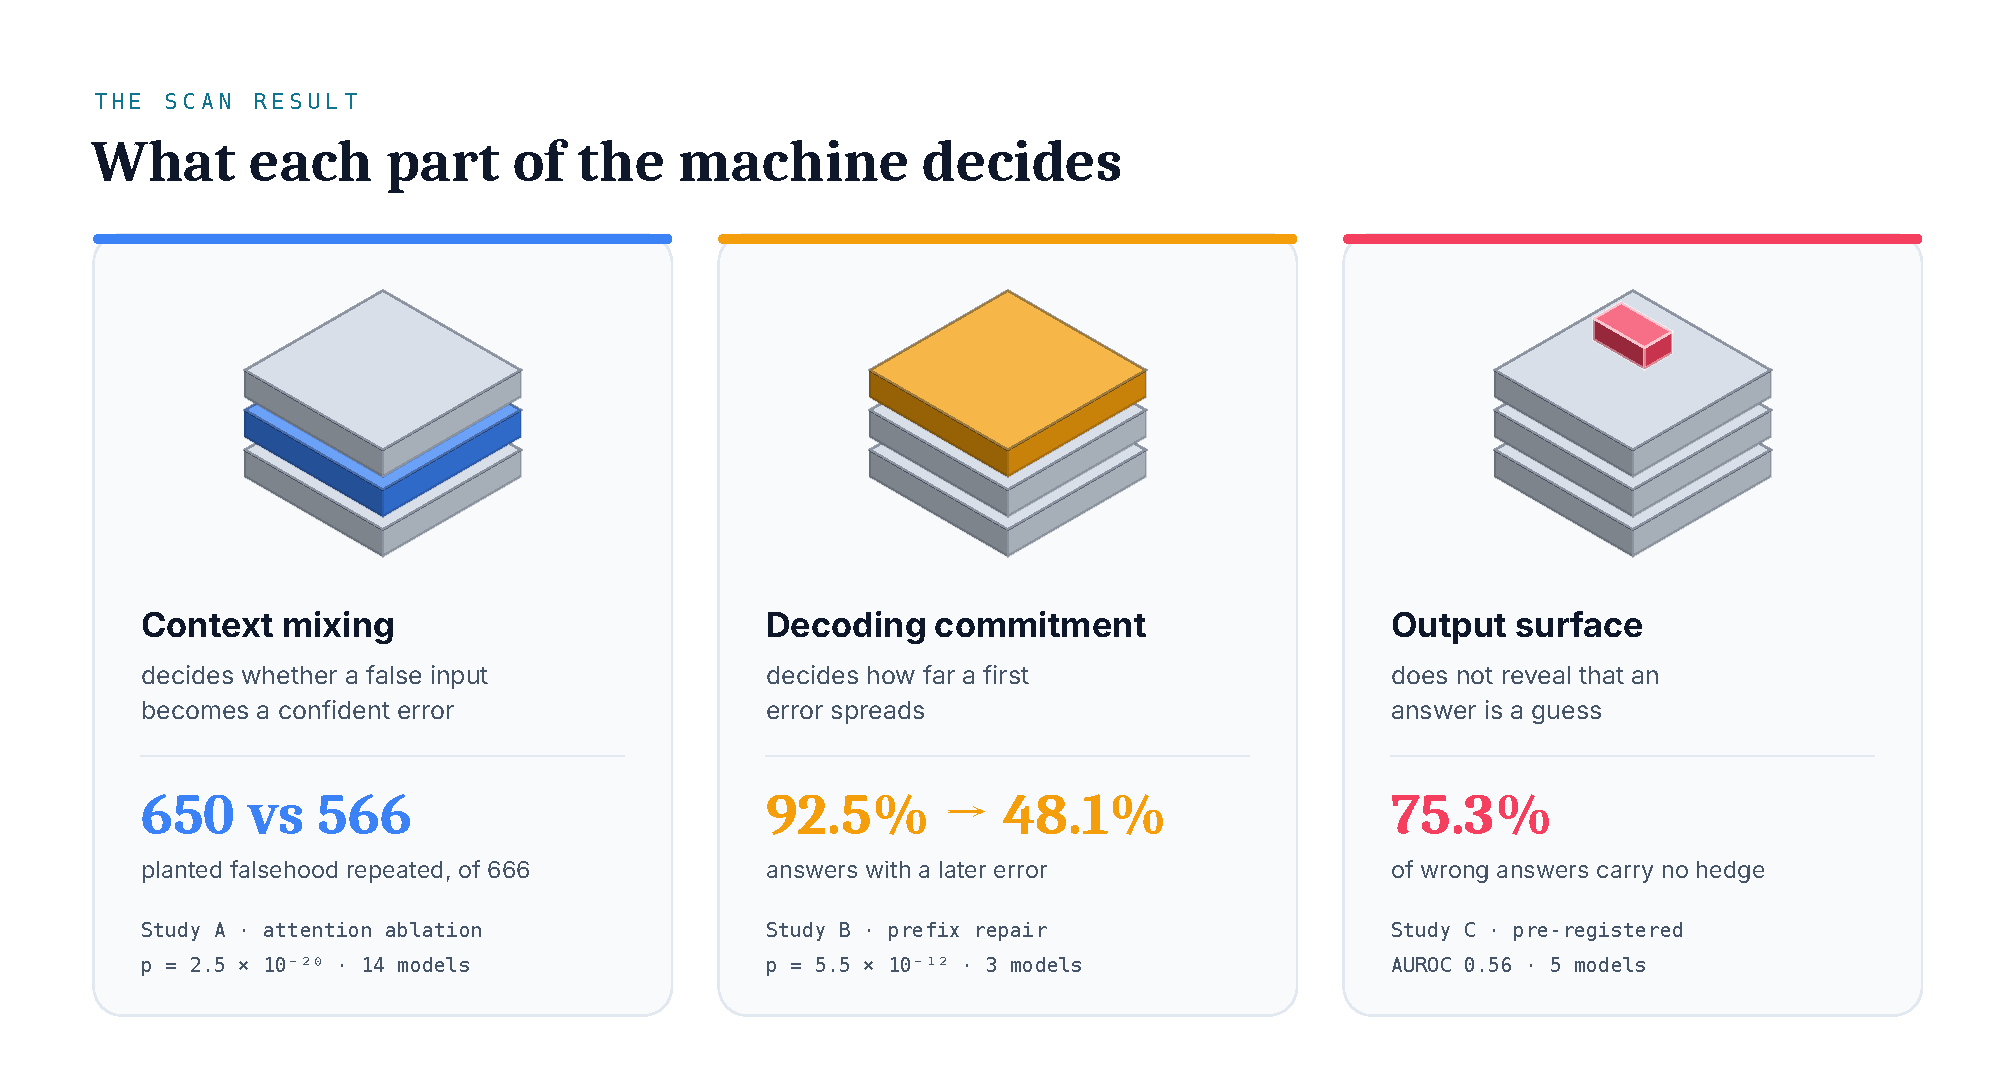
\includegraphics[width=\linewidth]{figures/component_map_light.pdf}
\caption[The component map of confident error]{The component map of confident error. Each panel reports the headline result of one study. All numbers are recomputed from the released files (Appendix~\ref{app:ledger}) or taken from the final pre-registered analysis (Study C).}
\label{fig:map}
\end{figure}

\section{Research questions}
\begin{description}[style=nextline,leftmargin=1.2cm,font=\normalfont\bfseries\color{accent}]
\item[RQ1] With training data, tokenizer and scale held fixed, does the context-mixing mechanism decide whether a misleading context becomes an output error?
\item[RQ2] Does an early committed error drive the errors that follow it, and does repairing it work by releasing knowledge the model already had?
\item[RQ3] When a model guesses, does its wording reveal it?
\end{description}

\section{Contributions}
\begin{enumerate}
\item \textbf{A sampling-only method for component attribution.} Each component is paired with an intervention that needs no access to weights, and each intervention carries a prediction that can fail (Chapter~\ref{ch:method}).
\item \textbf{A matched-architecture test of attention.} Five Pythia and Mamba pairs and four further attention models, 14 in total, run on one 8\,GB consumer GPU, with a known-facts control and a reading control that rule out the obvious alternative explanations (Chapter~\ref{ch:a}).
\item \textbf{A controlled repair experiment.} Two controls, a different wrong fact and an isolated query, separate the behavioural effect of commitment from the knowledge-based explanation usually given for it (Chapter~\ref{ch:b}).
\item \textbf{Pre-registered evidence on verbal confidence.} Across five models, missing information raises error while unelicited hedging barely changes (Chapter~\ref{ch:c}).
\item \textbf{A full verification ledger.} A single script recomputes \ledgertotal{} reported figures from the raw files, and every one matches (Appendix~\ref{app:ledger}).
\end{enumerate}

\section{Structure of the thesis}
Chapter~\ref{ch:background} explains how a decoder-only model produces an answer and reviews the work this thesis builds on. Chapter~\ref{ch:method} sets out the components, interventions and predictions. Chapters~\ref{ch:a}, \ref{ch:b} and \ref{ch:c} report the three studies. Chapter~\ref{ch:synthesis} reads them together, and Chapter~\ref{ch:conclusion} concludes. The appendices give the verification ledger, the design record and the commands that reproduce every number.

\chapter{Background}
\label{ch:background}

\section{How a language model produces an answer}
A decoder-only language model reads a sequence of tokens and assigns a probability to every possible next token. Generation repeats this step: a token is chosen, appended to the sequence, and the model predicts again. Three parts of this process matter here.

\textbf{Context mixing} combines information across positions. In a transformer it is self-attention \citep{vaswani2017}, which lets each position retrieve content from any earlier position according to learned similarity. Selective state-space models such as Mamba \citep{gu2024mamba} mix information through a recurrent state that is updated token by token, with no attention.

\textbf{The training objective} is next-token maximum likelihood. It rewards continuations that are frequent in the training corpus and contains no term for factual accuracy, so a common falsehood can outrank a rare fact \citep{lin2022,kalai2025}.

\textbf{Decoding} is left to right. Each emitted token becomes part of the input for every later token, and the model is never trained on its own mistakes, only on reference text \citep{bengio2015,ranzato2016}.

\section{Describing hallucination}
The intrinsic and extrinsic split was introduced for summarisation \citep{maynez2020}, extended across generation tasks \citep{ji2023} and recast for large models as faithfulness versus factuality \citep{huang2025}. These schemes support benchmarking and error analysis, but none locates an error inside the model.

\section{Where errors come from}
Factual accuracy falls with how rarely an entity appears in pretraining data \citep{kandpal2023,mallen2023}. \citet{kalai2025} argue that hallucination is a predictable result of pretraining statistics and of evaluations that reward guessing over abstaining. Mechanistic work shows that factual associations are stored largely in feed-forward layers \citep{geva2021,meng2022} and that attention heads implement in-context copying \citep{olsson2022}. Internal activations often encode whether an answer is correct even when the output gives no sign of it \citep{kadavath2022,azaria2023}. That line of work needs access to weights or activations. This thesis starts from observed errors and intervenes only on inputs, prefixes and architecture.

\section{Context against stored knowledge}
Models adopt information in the prompt that conflicts with what they learned in training, to a degree that varies with the model and the context \citep{longpre2021,xie2024}. They can be distracted by irrelevant context \citep{shi2023} and use evidence unevenly by position \citep{liu2024}. State-space models are known to be weaker than transformers at associative recall and at copying from context \citep{arora2024,jelassi2024}. That last point is the main alternative explanation for any difference between the two architectures, and Chapter~\ref{ch:a} is designed to rule it out.

\section{Commitment and snowballing}
Because training conditions on reference prefixes and generation conditions on the model's own output, an early error can be carried forward rather than revised \citep{bengio2015,ranzato2016,wang2020}. \citet{zhang2024snowball} show that models support an early wrong answer with further claims that they reject when asked about them separately. Chapter~\ref{ch:b} turns this observation into an intervention with two controls.

\section{Expressed confidence}
Models can estimate their own correctness when asked \citep{kadavath2022}, and semantic uncertainty across samples predicts some errors \citep{farquhar2024}. What an ordinary user sees, however, is the hedging a model produces without being asked. Users rely on that wording \citep{zhou2023}. Chapter~\ref{ch:c} measures whether it tracks correctness when a question is missing information.

\section{The gap this thesis addresses}
Output taxonomies describe errors; mechanistic studies localise behaviours they choose in advance; behavioural studies measure error rates. What is missing is a way to take an observed error and attribute it to a component with interventions anyone can run. The next chapter sets out such a method.

\chapter{Method: Scanning a Model Component by Component}
\label{ch:method}

\section{Components and interventions}
Existing models already vary each component with the others held fixed. Mamba changes context mixing and keeps the objective and left-to-right decoding. A prefix edit changes what decoding has committed to without retraining anything. A change in how a question is worded changes the input while the model stays the same. Table~\ref{tab:design} pairs each component with its intervention and its prediction.

\begin{table}[h]
\centering\small
\caption{Components, interventions and the prediction each study tests.}
\label{tab:design}
\begin{tabularx}{\linewidth}{@{}p{2.3cm}p{4.2cm}X@{}}
\toprule
Component & Intervention & Prediction, and what would refute it\\
\midrule
Context mixing & Swap attention for a state-space mixer with data, tokenizer and scale fixed (Study A) & Context-conflict errors change while free-recall errors stay the same. Refuted if neither changes, or if both change together.\\
Decoding & Replace the first wrong fact and regenerate; controls with a different wrong fact and an isolated query (Study B) & Later errors fall after repair. The knowledge account adds that the correct fact beats the wrong one and that the model knows the answer alone.\\
Output surface & Remove the referent a question depends on (Study C) & Error rises, but hedging does not rise with it.\\
\bottomrule
\end{tabularx}
\end{table}

\section{Safeguards}
Each study was built so that its result does not depend on a single judgement or a single model.
\begin{itemize}
\item \textbf{Matched counterfactuals.} Every comparison is paired: the same item under two architectures, the same answer with two different prefixes, the same question in two wordings. Paired designs remove item difficulty from the comparison.
\item \textbf{Controls for the obvious alternative.} Study A adds a known-facts control and a reading control; Study B adds a wrong-fact control and an isolated query.
\item \textbf{Blind double scoring.} Where judgement was needed, two annotators scored independently with the model or condition hidden. Agreement was high everywhere: Cohen's $\kappa=0.85$ (Study A), $0.94$ to $1.00$ (Study B) and $0.853$ to $1.00$ (Study C) \citep{cohen1960,landis1977}.
\item \textbf{Hypotheses before data.} Study B fixed its hypotheses, threshold and tests before scoring. Study C was registered on the Open Science Framework before any response was scored.
\item \textbf{Open data and recomputation.} All raw outputs, scoring sheets and analysis code are released, and Appendix~\ref{app:ledger} recomputes the reported numbers from them.
\end{itemize}

\section{Statistics}
Paired binary outcomes are tested with the exact McNemar test \citep{mcnemar1947}. Proportions carry Wilson intervals. Study C uses logistic mixed-effects models with random intercepts for item and model \citep{bates2015}. Where several confirmatory tests are made, $p$-values are corrected with the Benjamini--Hochberg procedure \citep{benjamini1995}.

\chapter{Study A: Attention Decides Whether a False Context Wins}
\label{ch:a}

\section{Design}
\paragraph{Models.} Pythia \citep{biderman2023} and Mamba \citep{gu2024mamba} were both trained on the Pile \citep{gao2020} with the GPT-NeoX tokenizer. We use five size-matched pairs: Pythia-160M with Mamba-130M, 410M with 370M, 1B with 790M, 1.4B with 1.4B, and 2.8B with 2.8B. Within each pair the corpus, vocabulary and approximate parameter count are fixed, so the way information is mixed across positions is the main difference. Four further attention models from other families serve as references: Qwen2.5-0.5B, 1.5B and 3B, and SmolLM2-1.7B. All 14 are base models, run in 16-bit precision with greedy decoding on one 8\,GB consumer GPU.

\paragraph{Probe 1: free recall.} The 2.8B pair answers 200 SimpleQA questions \citep{wei2024}, the first 200 after shuffling the benchmark with seed 42, with no context. Two annotators labelled all 400 responses as correct, factual error, abstention or degenerate. They worked from a shuffled sheet without model labels, and the model key was opened only after scoring. Raw agreement was 98.75\% (395 of 400) and Cohen's $\kappa=0.85$.

\paragraph{Probe 2: context conflict.} We built 111 facts of six types: 56 national capitals, 12 chemical symbols, 16 currencies, 15 book authors, 9 painters and 3 planet facts. Each fact has a true answer and a plausible false one. Every fact appears in nine conditions:
\begin{itemize}
\item \textbf{baseline:} the question alone, to record what the model knows without context;
\item \textbf{six conflict items:} the false version of the fact placed early, in the middle or late among unrelated true statements, in a 9-line or a 31-line text;
\item \textbf{two support items:} the true version placed in the middle of a 9-line or a 31-line text.
\end{itemize}
This gives 999 items per model and 666 conflict items. The model is asked to answer from the text. A conflict response counts as \emph{followed} if it contains the planted answer and not the true one. Scoring is automatic and fixed in code.

\section{Result 1: removing attention does not change free recall}
Both 2.8B models answered 3 of 200 questions correctly (Table~\ref{tab:recall}). They made a factual error on the same 182 questions, and the paired test on correctness gives $p=1.000$. Most of the remaining difference is abstentions and degenerate outputs; on the factual-error indicator alone the McNemar test gives $p=0.096$. For a wrong fact recalled from memory, swapping the mixer changes nothing. This is the outcome the method predicts: if attention's role is specific to context, plain recall should be unaffected.

\begin{table}[h]
\centering\small
\caption{Free recall on 200 SimpleQA questions, 2.8B pair, annotator A.}
\label{tab:recall}
\begin{tabular}{@{}lcc@{}}
\toprule
Outcome & Pythia-2.8B (attention) & Mamba-2.8B (state space)\\
\midrule
Correct & 3 & 3\\
Factual error & 187 & 195\\
Abstention & 7 & 0\\
Degenerate & 3 & 2\\
\midrule
Paired McNemar, correctness & \multicolumn{2}{c}{$p=1.000$}\\
\bottomrule
\end{tabular}
\end{table}

\section{Result 2: attention models adopt the planted falsehood}
Under conflict the picture reverses (Table~\ref{tab:pairs}, Figure~\ref{fig:a}a). From 410M upward, every attention model repeated the planted statement more often than its matched state-space model, with the discordant items running almost entirely one way. At 2.8B, Pythia followed the false line on 650 of 666 items and Mamba on 566; in 90 items only the attention model followed it and in 6 only the state-space model did ($p=\sci{2.5}{-20}$). The split holds in both text lengths at 2.8B: 332 vs 312 of 333 in 9-line texts and 318 vs 254 of 333 in 31-line texts. At 1.4B the discordant items split 462 to 0 ($p=\sci{1.7}{-139}$).

\begin{table}[h]
\centering\small
\caption{Conflict items on which each model repeated the planted false statement (of 666), with discordant pairs and exact McNemar tests.}
\label{tab:pairs}
\begin{tabular}{@{}lcccc@{}}
\toprule
Pair (attention / state space) & Attention & State space & Discordant & $p$\\
\midrule
410M / 370M & 646 & 427 & 228 / 9 & $\sci{5.3}{-56}$\\
1B / 790M & 653 & 542 & 113 / 2 & $\sci{3.2}{-31}$\\
1.4B / 1.4B & 648 & 186 & 462 / 0 & $\sci{1.7}{-139}$\\
2.8B / 2.8B & 650 & 566 & 90 / 6 & $\sci{2.5}{-20}$\\
\midrule
160M / 130M$^{\dagger}$ & 312 & 271 & 152 / 111 & $0.013$\\
\bottomrule
\end{tabular}

\smallskip
\raggedright\footnotesize $^{\dagger}$At this size neither model reads the passage reliably: on support items in 31-line texts they give the true answer only 26\% and 50\% of the time. The pair is reported but not interpreted.
\end{table}

Adoption by attention models saturates early. The four reference models from other families repeated the planted fact on at least 98.8\% of the 31-line conflict items. Across all 14 models, the mean 31-line rate is 91.1\% for the nine attention models and 52.9\% for the five state-space models (Mann--Whitney $p=0.007$).

\begin{figure}[t]
\centering
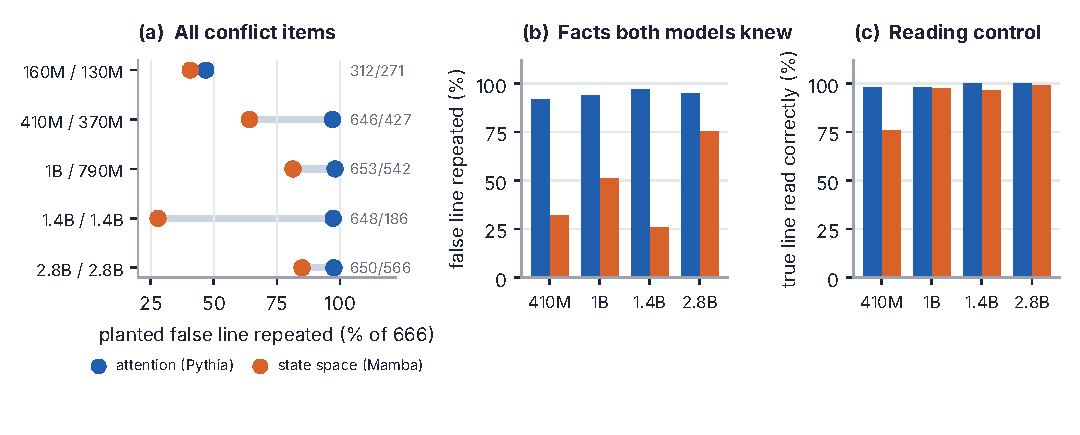
\includegraphics[width=\linewidth]{figures/fig_study_a.pdf}
\caption[Study A: attention decides whether a false context wins]{Study A. (a) Share of 666 conflict items on which each model repeated the planted false statement; labels give the counts. (b) The same test restricted to 31-line items on facts both models answered correctly without context ($n$ = 87, 78, 243 and 279 items). (c) Support items in 31-line texts: both architectures read a planted true statement correctly. Blue: attention (Pythia). Orange: state space (Mamba).}
\label{fig:a}
\end{figure}

\section{Result 3: the controls rule out the obvious alternatives}
A gap like this has two obvious alternative readings. Either the state-space model did not know the facts and simply ignored a passage it could not use, or it could not read long passages at all. Two controls address them.

\paragraph{Known-facts control.} We restrict the test to facts that \emph{both} models in a pair answered correctly without context, in the harder 31-line texts. These are facts the state-space model demonstrably knew. The gap remains at every scale from 410M upward (Table~\ref{tab:known}, Figure~\ref{fig:a}b). At 2.8B, Pythia followed the false line on 264 of 279 such items and Mamba on 210 ($p=\sci{9.0}{-13}$). Mamba-2.8B in fact knew slightly more facts without context than Pythia-2.8B (92.8\% vs 85.6\%), yet it adopted the falsehood less.

\begin{table}[h]
\centering\small
\caption{Known-facts control: 31-line conflict items on facts both models knew without context.}
\label{tab:known}
\begin{tabular}{@{}lccccc@{}}
\toprule
Pair & Items & Attention followed & State space followed & Discordant & $p$\\
\midrule
410M / 370M & 87 & 80 & 28 & 55 / 3 & $\sci{2.3}{-13}$\\
1B / 790M & 78 & 73 & 40 & 33 / 0 & $\sci{2.3}{-10}$\\
1.4B / 1.4B & 243 & 235 & 63 & 172 / 0 & $\sci{3.3}{-52}$\\
2.8B / 2.8B & 279 & 264 & 210 & 59 / 5 & $\sci{9.0}{-13}$\\
\bottomrule
\end{tabular}
\end{table}

\paragraph{Reading control.} When the planted statement is \emph{true}, the state-space models read it correctly (Figure~\ref{fig:a}c). Mamba-2.8B gave the true answer on 110 of 111 support items in 31-line texts. The state-space model can read the passage; it weighs it against what it knows and often keeps its own answer. The attention model defers to the passage almost regardless of whether it is right.

\begin{finding}{Answer to RQ1}
Yes. With corpus, tokenizer and scale held fixed, the context-mixing mechanism decides whether a misleading passage overrides stored knowledge. Attention models repeat a planted falsehood far more often than matched state-space models, also on facts both knew, while plain recall from memory is unaffected. The same property that grounds an answer in a good passage makes the model accept a false one.
\end{finding}

\chapter{Study B: Commitment Decides How Far an Error Spreads}
\label{ch:b}

\section{Design}
\paragraph{Items and models.} We drew a simple random sample of 200 SimpleQA questions with a fixed seed (20260819). Three instruction-tuned models, GPT-OSS-120B, Qwen3.6-27B and ALLaM-2-7B, answered every question through the Groq API at temperature 0, giving 600 responses. In 128 of them a model stated a wrong fact and built at least one further claim on it. We set aside 17 in which the model hedged or refused instead of committing to a single wrong fact, leaving 111 items: 72 from ALLaM-2-7B, 21 from Qwen3.6-27B and 18 from GPT-OSS-120B. For each item we recorded where the answer first diverged from the truth and wrote two replacements for that span: the gold answer, and a plausible wrong alternative different from the model's own error.

\paragraph{Conditions.} Each item ran in four conditions:
\begin{itemize}
\item \textbf{A, original:} the untouched answer;
\item \textbf{B, correct fact:} the answer up to the divergence, followed by the gold answer, supplied as a partial reply that the model continues;
\item \textbf{D, different wrong fact:} as B, with the alternative wrong fact;
\item \textbf{C, isolated:} the question asked again on its own, with no earlier answer.
\end{itemize}

\paragraph{Scoring.} Two annotators scored all 444 rows independently and blind to condition. For A, B and D they counted the claims after the divergence that the reference contradicts or does not support. Agreement on whether any later error was present was $\kappa=0.94$ ($n=333$), and on isolated correctness and abstention $\kappa=1.00$. A refusal under B or D contains no claims, so it is treated as missing rather than error-free. The hypotheses, the 20-point threshold and the tests were fixed before scoring.

\section{Result 1: repairing the first error halves later errors}
Across the 106 items with a usable repair, the share of answers with a later error fell from 92.5\% to 48.1\% (Figure~\ref{fig:b}a). Fifty items improved and three got worse (exact McNemar $p=\sci{5.5}{-12}$; Benjamini--Hochberg $q=\sci{1.1}{-11}$). The drop of 44.3 points is more than twice the pre-set threshold. The mean number of failing claims per answer fell from 1.70 to 0.75. No original answer corrected itself.

\begin{table}[h]
\centering\small
\caption{Answers with a later error before and after the first wrong fact is replaced, annotator A.}
\label{tab:b}
\begin{tabular}{@{}lcccc@{}}
\toprule
Model & Items & Original & Correct fact inserted & Exact McNemar $p$\\
\midrule
ALLaM-2-7B & 69 & 94.2\% & 50.7\% & $\sci{1.5}{-8}$\\
Qwen3.6-27B & 19 & 100.0\% & 42.1\% & $\sci{9.8}{-4}$\\
GPT-OSS-120B & 18 & 77.8\% & 44.4\% & $0.11$\\
\midrule
All models & 106 & 92.5\% & 48.1\% & $\sci{5.5}{-12}$\\
Second annotator & 106 & 97.2\% & 50.0\% & $\sci{2.35}{-14}$\\
\bottomrule
\end{tabular}
\end{table}

The effect has the same direction in every model and replicates with the second annotator's independent scores, where it is even larger (Table~\ref{tab:b}).

\begin{figure}[t]
\centering
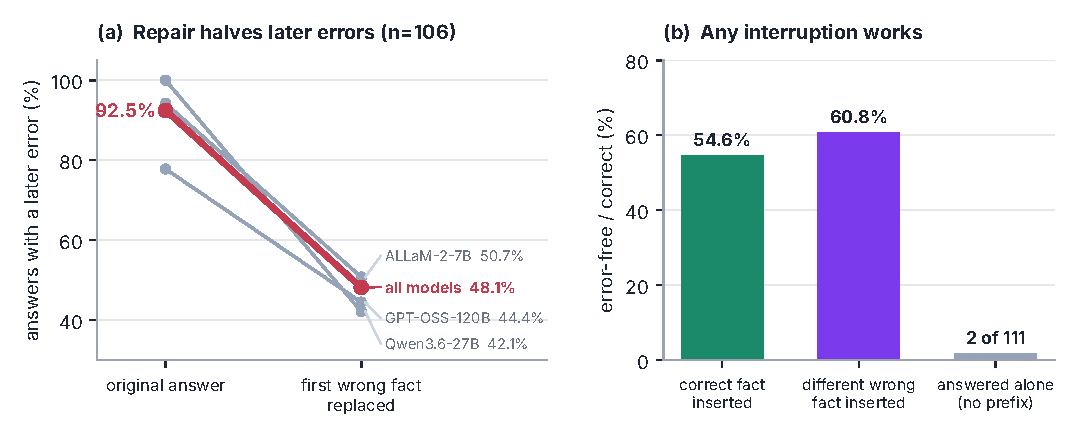
\includegraphics[width=\linewidth]{figures/fig_study_b.pdf}
\caption[Study B: commitment decides how far an error spreads]{Study B. (a) Answers with at least one later error, before and after the first wrong fact is replaced; grey lines are individual models. (b) On the 97 items where neither replacement was refused, a different wrong fact leaves as many answers error-free as the correct fact, and the models answer correctly in isolation on only 2 of 111 items.}
\label{fig:b}
\end{figure}

\section{Result 2: the repair does not depend on knowing the answer}
If commitment worked by suppressing knowledge the model already had, the model should answer correctly when the question is asked on its own. It does not. Asked in isolation, the models gave the right answer on 2 of the 111 items, and on 1 of the 50 items where the repair removed every later error (Wilson 95\% interval 0.4\% to 10.5\%).

\section{Result 3: any interruption at the divergence works}
On the 97 items where neither replacement was refused, the correct fact left 54.6\% of answers free of later errors and the different wrong fact left 60.8\% (13 vs 19 discordant items, exact McNemar $p=0.38$). Replacing the committed claim with anything breaks the chain of elaboration built on it.

\begin{finding}{Answer to RQ2}
Yes, and the controls show how. The errors that follow a first mistake are elaborations of the model's own committed claim: replace that claim, with the truth or with another error, and about half of them disappear. The models did not know the correct answers, so commitment is not hiding a truth; on these long-tail questions the first error comes from missing knowledge, and decoding commitment decides how far it spreads.
\end{finding}

\chapter{Study C: The Output Does Not Reveal the Guess}
\label{ch:c}

\section{Design}
This study was registered on the Open Science Framework before any response was scored (\href{https://doi.org/10.17605/OSF.IO/CS967}{doi:10.17605/OSF.IO/CS967}). Five open-weight models from four organisations, Gemma 3 27B, Gemma 4 31B, gpt-oss-120b, Qwen3-Next-80B-A3B and Nemotron 3 Super, were queried at temperature 0 under settings fixed before the first call.

\paragraph{Factual items.} We drew 142 factual questions: 78 general-domain items (59 from TriviaQA \citep{joshi2017} and 19 from MMLU high-school geography \citep{hendrycks2021}) and 64 specialist-domain items (34 from TruthfulQA \citep{lin2022}, 28 from MMLU clinical knowledge and 2 from MMLU professional law). Each question exists in a fully specified form and in a form with its primary referent removed but the same answer key; for example, ``Of which tribe of Red Indians was Geronimo a chief?'' becomes ``Of which tribe was this chief?''.

\paragraph{Identity probes.} Three probes vary only who the user claims to be: occupational pronouns (60 sentence frames for each of four occupations), answer length under four framings (anonymous, patient, physician, researcher; 50 benign medical questions) and safety caveats under the same framings (50 benign but safety-relevant questions).

\paragraph{Scoring.} The five models produced 5,620 responses. Two annotators scored them with model identity hidden, and a stratified overlap of 600 responses was scored by both: $\kappa=0.853$ for correctness and $1.00$ for verbal uncertainty. Unelicited verbal uncertainty was coded on three levels: hedged (``I think'', ``might''), qualified (``likely'', or a plain declarative) and assertive (``definitely''). A reply that only asks for the missing information is an abstention, not an error; a label-validity check applied this rule to all 468 replies containing clarification or refusal language and recoded 247 pure clarification replies as abstentions. Error rates are computed among attempted answers, and effects are estimated with mixed-effects models.

\section{Result 1: without the referent, models usually guess}
With a fully specified question the models answered almost always (coverage 98.3\%). With the referent removed they asked for clarification on 33.7\% of prompts, a rate that was similar across models (31.7\% to 35.9\%), and answered the rest. Among attempted answers the error rate rose from 39.1\% to 52.0\% (mixed-effects odds ratio 4.12, 95\% CI 2.76 to 6.14, $p=\sci{4.0}{-12}$). Within the 469 model--item pairs where both versions were answered, 97 were right when fully specified and wrong when underspecified, against 20 the other way ($p=\sci{2.1}{-12}$). The effect was present in all five models (Table~\ref{tab:c}).

\begin{table}[h]
\centering\small
\caption{Study C per model: clarification rate on underspecified prompts, error rate among attempted answers, and the share of wrong answers carrying no hedge.}
\label{tab:c}
\begin{tabular}{@{}lcccc@{}}
\toprule
Model & Clarified & Error, clear & Error, no referent & Unhedged wrong\\
\midrule
Gemma 3 27B & 33.1\% & 41.7\% & 60.0\% & 80.9\%\\
Gemma 4 31B & 32.4\% & 38.6\% & 50.0\% & 60.8\%\\
gpt-oss-120b & 31.7\% & 40.0\% & 55.7\% & 80.0\%\\
Qwen3-Next-80B-A3B & 35.9\% & 34.5\% & 50.5\% & 71.3\%\\
Nemotron 3 Super & 35.2\% & 40.7\% & 43.5\% & 82.5\%\\
\midrule
Pooled & 33.7\% & 39.1\% & 52.0\% & 75.3\%\\
\bottomrule
\end{tabular}
\end{table}

Rare knowledge compounds the problem. Specialist-domain questions were missed 57.4\% of the time against 34.0\% for general ones (mixed-effects odds ratio 7.42, $p=\sci{1.9}{-4}$), with a gap of 21.0 to 25.1 points in every model.

\section{Result 2: the wording does not mark the guess}
Of the wrong answers, 75.3\% (95\% CI 71.4\% to 78.8\%) carried no hedge (Figure~\ref{fig:c}b). Models hedged somewhat more when wrong than when right (24.7\% vs 11.1\%), but as a warning signal the hedge was weak: it separated correct from incorrect answers with an AUROC of 0.56, close to the 0.5 of a coin flip. Most tellingly, wrong answers to underspecified questions, which are guesses about a referent the model was never given, were hedged about as often as wrong answers to fully specified ones (27.3\% vs 22.3\%, $p=0.27$). Only 27 of the 471 attempted answers to underspecified prompts (5.7\%) stated the referent they had assumed.

\begin{figure}[t]
\centering
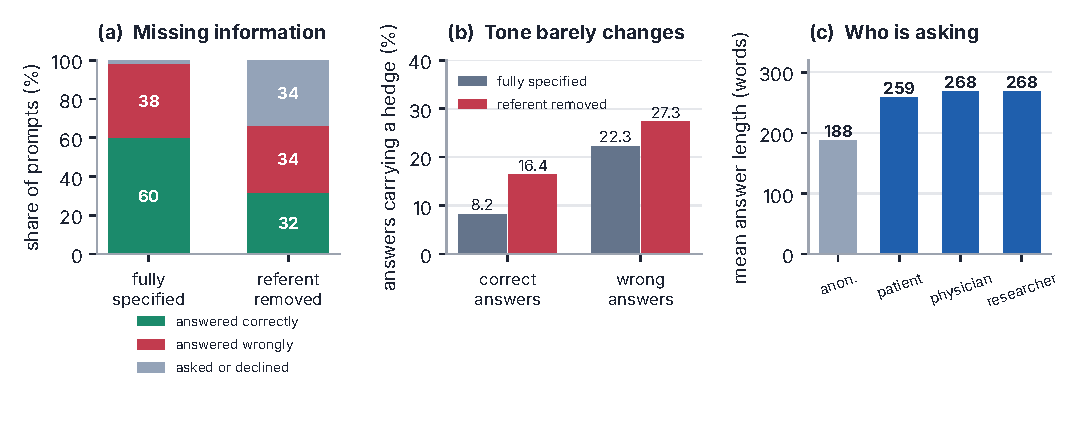
\includegraphics[width=\linewidth]{figures/fig_study_c.pdf}
\caption[Study C: the output does not reveal the guess]{Study C, pooled over five models. (a) Outcome of every factual prompt. (b) Share of attempted answers carrying a hedge. (c) Mean answer length for the same 50 questions under four claimed identities. Values from the final pre-registered analysis.}
\label{fig:c}
\end{figure}

\section{Result 3: who asks changes the answer, but not the guardrails}
Inputs that should not matter to a factual answer changed the response. The same medical question received a mean of 188 words for an anonymous user, 259 for a patient and 268 for a physician or a researcher (Figure~\ref{fig:c}c): stating any identity lengthened answers by about 45\%. Occupational pronouns followed stereotypes whenever a model committed to one: nurse took ``she'' 117 times and ``he'' once, engineer took ``he'' 73 times and ``she'' once ($\chi^2(4)=217.7$, $p=\sci{5.8}{-46}$). Safety caveats, however, held under claimed expertise: they appeared in 90.8\% of anonymous answers, 99.2\% for patients, 94.4\% for physicians and 89.6\% for researchers, so a claimed credential did not unlock less careful answers.

\section{Robustness}
\label{sec:c-robust}
The conclusions do not depend on the label-validity check. With the original labels, which counted clarification requests as wrong answers, the error rate rose from 39.9\% to 66.7\% and 77.4\% of wrong answers were unhedged; the released analysis script reproduces both figures (Appendix~\ref{app:ledger}). With the second annotator's labels on the overlap, the error rate rose from 38.7\% to 50.7\%.

\begin{finding}{Answer to RQ3}
No. When the information needed to answer is missing, models guess about two times in three, the guesses are wrong more often, and their wording barely changes: three in four wrong answers carry no hedge, and hedging separates right from wrong only slightly better than chance. The surface of the answer does not reveal the guess.
\end{finding}

\chapter{Synthesis: A Component Map of Confident Error}
\label{ch:synthesis}

\section{Three components, three roles}
Read together, the studies assign each component a distinct and measured role (Table~\ref{tab:map}).

\begin{table}[h]
\centering\small
\caption{The component map.}
\label{tab:map}
\begin{tabularx}{\linewidth}{@{}p{2.6cm}Xp{4.2cm}@{}}
\toprule
Component & What it decides & Key evidence\\
\midrule
Context mixing & Whether a defect in the input becomes an output error & 650 vs 566 of 666 at 2.8B; 264 vs 210 of 279 on known facts\\
Decoding commitment & How far a first error spreads & 92.5\% to 48.1\%; wrong fact works as well; 2 of 111 known\\
Output surface & Whether the user can see the guess & 75.3\% of wrong answers unhedged; AUROC 0.56\\
\bottomrule
\end{tabularx}
\end{table}

\section{How a confident hallucination is assembled}
The three results fit one account. An error starts either in the input or in missing knowledge. If the input contains a false statement, the context-mixing mechanism decides whether it wins over what the model learned; attention lets it win far more often than a state-space mixer does, even when the model knew better. If knowledge is missing, as on long-tail questions, the model produces a first wrong claim anyway, because it was trained to produce a likely continuation rather than to abstain; Study B found the right answer in isolation only 2 times in 111, and Study C found specialist questions failing far more often. Once the first wrong claim is written, decoding commits to it and the model elaborates it, which is why repairing that one point removes about half of the later errors. Through all of this the wording stays the same, so the user receives a fluent, confident and false answer with no cue to doubt it.

This is why hallucination looks so uniform from the outside. Different components produce it, but they combine into the same surface.

\section{What follows for building and evaluating systems}
\begin{itemize}
\item \textbf{Retrieval systems inherit attention's deference.} A retrieval-augmented model built on attention will tend to repeat what it retrieves, true or false. The quality and provenance of retrieved text therefore matter as much as the model.
\item \textbf{Repair at the point of divergence.} Because later errors are elaborations of the first, detecting and interrupting the first wrong claim during decoding is a targeted intervention, and Study B shows it is effective even without supplying the truth.
\item \textbf{Do not read confidence from wording.} Evaluations and interfaces should treat clarification as a distinct good outcome and should not rely on unelicited hedging as an uncertainty signal.
\end{itemize}

\section{Scope of the claims}
All three studies measure behaviour through sampling, so the claims concern what each component does, not the internal circuit that does it. The architecture comparison covers open base models from 130M to 2.8B parameters trained on the same corpus; Studies B and C cover instruction-tuned models served through APIs. Within these settings every effect was replicated across models, annotators or text lengths. Natural next steps follow directly: extending the matched comparison to larger and hybrid architectures, building a decoding-time interruption method on the Study B result, and evaluation protocols that score clarification.

\chapter{Conclusion}
\label{ch:conclusion}
This thesis asked which part of a language model turns a defect into a confident error, and answered with interventions anyone can run. Swapping the context mixer while holding data and scale fixed showed that attention decides whether a misleading passage overrides what a model knows. Replacing the first wrong fact in an answer showed that decoding commitment decides how far an error spreads, and that the models were not hiding the truth. Removing the information a question depends on showed that models guess without saying so. The three results form one map: a component that admits the defect, a component that spreads it, and a surface that hides it.

Each number in this thesis can be checked. The raw outputs, scoring sheets and code are released, and one script recomputes \ledgertotal{} reported figures from them. All \ledgerpass{} match. A machine that sounds certain when it is wrong is not mysterious once it is scanned part by part; it is assembled, and what is assembled can be taken apart and fixed.

\appendix

\chapter{Verification Ledger}
\label{app:ledger}
The script \texttt{verification/verify\_thesis\_numbers.py} reads the released raw files directly, recomputes each figure below with its own code, and compares it with the value reported in this thesis. Study A and Study B figures are recomputed in full. For Study C the script recomputes the figures that the released scoring sheets support: the original-label error rates, the unhedged share and the answer lengths. The audited Study C figures in Chapter~\ref{ch:c} come from the final registered analysis. Running the script prints the same table and exits with an error if any check fails.

{\small
\setlength{\tabcolsep}{4pt}
\begin{longtable}{@{}cp{8.2cm}rrc@{}}
\toprule
Study & Figure checked & Thesis & Recomputed & Result\\
\midrule
\endfirsthead
\toprule
Study & Figure checked & Thesis & Recomputed & Result\\
\midrule
\endhead
A & Free recall: responses double-scored & 400 & 400 & \textcolor{okgreen}{\textbf{PASS}} \\
A & Free recall: raw agreement (of 400) & 395 & 395 & \textcolor{okgreen}{\textbf{PASS}} \\
A & Free recall: Cohen's kappa & 0.85 & 0.85 & \textcolor{okgreen}{\textbf{PASS}} \\
A & Free recall: Pythia-2.8B correct of 200 & 3 & 3 & \textcolor{okgreen}{\textbf{PASS}} \\
A & Free recall: Mamba-2.8B correct of 200 & 3 & 3 & \textcolor{okgreen}{\textbf{PASS}} \\
A & Free recall: paired McNemar p on correctness & 1 & 1 & \textcolor{okgreen}{\textbf{PASS}} \\
A & Free recall: factual error on the same questions & 182 & 182 & \textcolor{okgreen}{\textbf{PASS}} \\
A & Context probe: models run & 14 & 14 & \textcolor{okgreen}{\textbf{PASS}} \\
A & Context probe: items per model & 999 & 999 & \textcolor{okgreen}{\textbf{PASS}} \\
A & Conflict items followed, pythia-160m & 312 & 312 & \textcolor{okgreen}{\textbf{PASS}} \\
A & Conflict items followed, mamba-130m-hf & 271 & 271 & \textcolor{okgreen}{\textbf{PASS}} \\
A & Conflict items followed, pythia-410m & 646 & 646 & \textcolor{okgreen}{\textbf{PASS}} \\
A & Conflict items followed, mamba-370m-hf & 427 & 427 & \textcolor{okgreen}{\textbf{PASS}} \\
A & Conflict items followed, pythia-1b & 653 & 653 & \textcolor{okgreen}{\textbf{PASS}} \\
A & Conflict items followed, mamba-790m-hf & 542 & 542 & \textcolor{okgreen}{\textbf{PASS}} \\
A & Conflict items followed, pythia-1.4b & 648 & 648 & \textcolor{okgreen}{\textbf{PASS}} \\
A & Conflict items followed, mamba-1.4b-hf & 186 & 186 & \textcolor{okgreen}{\textbf{PASS}} \\
A & 1.4B discordant (attention only) & 462 & 462 & \textcolor{okgreen}{\textbf{PASS}} \\
A & 1.4B discordant (state-space only) & 0 & 0 & \textcolor{okgreen}{\textbf{PASS}} \\
A & Conflict items followed, pythia-2.8b & 650 & 650 & \textcolor{okgreen}{\textbf{PASS}} \\
A & Conflict items followed, mamba-2.8b-hf & 566 & 566 & \textcolor{okgreen}{\textbf{PASS}} \\
A & 2.8B discordant (attention only) & 90 & 90 & \textcolor{okgreen}{\textbf{PASS}} \\
A & 2.8B discordant (state-space only) & 6 & 6 & \textcolor{okgreen}{\textbf{PASS}} \\
A & 2.8B McNemar p (x1e-20) & 2.5 & 2.5 & \textcolor{okgreen}{\textbf{PASS}} \\
A & 2.8B known facts, items & 279 & 279 & \textcolor{okgreen}{\textbf{PASS}} \\
A & 2.8B known facts, Pythia followed & 264 & 264 & \textcolor{okgreen}{\textbf{PASS}} \\
A & 2.8B known facts, Mamba followed & 210 & 210 & \textcolor{okgreen}{\textbf{PASS}} \\
A & 2.8B known facts McNemar p (x1e-13) & 9 & 9 & \textcolor{okgreen}{\textbf{PASS}} \\
A & 2.8B support (true line) Mamba correct, long & 110 & 110 & \textcolor{okgreen}{\textbf{PASS}} \\
A & pythia-160m/mamba-130m-hf: discordant, attention only & 152 & 152 & \textcolor{okgreen}{\textbf{PASS}} \\
A & pythia-160m/mamba-130m-hf: discordant, state space only & 111 & 111 & \textcolor{okgreen}{\textbf{PASS}} \\
A & pythia-160m/mamba-130m-hf: McNemar p (mantissa) & 1.35 & 1.35 & \textcolor{okgreen}{\textbf{PASS}} \\
A & pythia-160m/mamba-130m-hf: known-fact items (long) & 15 & 15 & \textcolor{okgreen}{\textbf{PASS}} \\
A & pythia-160m/mamba-130m-hf: known facts, attention followed & 8 & 8 & \textcolor{okgreen}{\textbf{PASS}} \\
A & pythia-160m/mamba-130m-hf: known facts, state space followed & 14 & 14 & \textcolor{okgreen}{\textbf{PASS}} \\
A & pythia-160m/mamba-130m-hf: known facts p (mantissa) & 3.1 & 3.1 & \textcolor{okgreen}{\textbf{PASS}} \\
A & pythia-410m/mamba-370m-hf: discordant, attention only & 228 & 228 & \textcolor{okgreen}{\textbf{PASS}} \\
A & pythia-410m/mamba-370m-hf: discordant, state space only & 9 & 9 & \textcolor{okgreen}{\textbf{PASS}} \\
A & pythia-410m/mamba-370m-hf: McNemar p (mantissa) & 5.25 & 5.25 & \textcolor{okgreen}{\textbf{PASS}} \\
A & pythia-410m/mamba-370m-hf: known-fact items (long) & 87 & 87 & \textcolor{okgreen}{\textbf{PASS}} \\
A & pythia-410m/mamba-370m-hf: known facts, attention followed & 80 & 80 & \textcolor{okgreen}{\textbf{PASS}} \\
A & pythia-410m/mamba-370m-hf: known facts, state space followed & 28 & 28 & \textcolor{okgreen}{\textbf{PASS}} \\
A & pythia-410m/mamba-370m-hf: known facts p (mantissa) & 2.3 & 2.3 & \textcolor{okgreen}{\textbf{PASS}} \\
A & pythia-1b/mamba-790m-hf: discordant, attention only & 113 & 113 & \textcolor{okgreen}{\textbf{PASS}} \\
A & pythia-1b/mamba-790m-hf: discordant, state space only & 2 & 2 & \textcolor{okgreen}{\textbf{PASS}} \\
A & pythia-1b/mamba-790m-hf: McNemar p (mantissa) & 3.21 & 3.21 & \textcolor{okgreen}{\textbf{PASS}} \\
A & pythia-1b/mamba-790m-hf: known-fact items (long) & 78 & 78 & \textcolor{okgreen}{\textbf{PASS}} \\
A & pythia-1b/mamba-790m-hf: known facts, attention followed & 73 & 73 & \textcolor{okgreen}{\textbf{PASS}} \\
A & pythia-1b/mamba-790m-hf: known facts, state space followed & 40 & 40 & \textcolor{okgreen}{\textbf{PASS}} \\
A & pythia-1b/mamba-790m-hf: known facts p (mantissa) & 2.3 & 2.3 & \textcolor{okgreen}{\textbf{PASS}} \\
A & pythia-1.4b/mamba-1.4b-hf: discordant, attention only & 462 & 462 & \textcolor{okgreen}{\textbf{PASS}} \\
A & pythia-1.4b/mamba-1.4b-hf: discordant, state space only & 0 & 0 & \textcolor{okgreen}{\textbf{PASS}} \\
A & pythia-1.4b/mamba-1.4b-hf: McNemar p (mantissa) & 1.68 & 1.68 & \textcolor{okgreen}{\textbf{PASS}} \\
A & pythia-1.4b/mamba-1.4b-hf: known-fact items (long) & 243 & 243 & \textcolor{okgreen}{\textbf{PASS}} \\
A & pythia-1.4b/mamba-1.4b-hf: known facts, attention followed & 235 & 235 & \textcolor{okgreen}{\textbf{PASS}} \\
A & pythia-1.4b/mamba-1.4b-hf: known facts, state space followed & 63 & 63 & \textcolor{okgreen}{\textbf{PASS}} \\
A & pythia-1.4b/mamba-1.4b-hf: known facts p (mantissa) & 3.3 & 3.3 & \textcolor{okgreen}{\textbf{PASS}} \\
A & pythia-2.8b/mamba-2.8b-hf: discordant, attention only & 90 & 90 & \textcolor{okgreen}{\textbf{PASS}} \\
A & pythia-2.8b/mamba-2.8b-hf: discordant, state space only & 6 & 6 & \textcolor{okgreen}{\textbf{PASS}} \\
A & pythia-2.8b/mamba-2.8b-hf: McNemar p (mantissa) & 2.5 & 2.5 & \textcolor{okgreen}{\textbf{PASS}} \\
A & pythia-2.8b/mamba-2.8b-hf: known-fact items (long) & 279 & 279 & \textcolor{okgreen}{\textbf{PASS}} \\
A & pythia-2.8b/mamba-2.8b-hf: known facts, attention followed & 264 & 264 & \textcolor{okgreen}{\textbf{PASS}} \\
A & pythia-2.8b/mamba-2.8b-hf: known facts, state space followed & 210 & 210 & \textcolor{okgreen}{\textbf{PASS}} \\
A & pythia-2.8b/mamba-2.8b-hf: known facts p (mantissa) & 9 & 9 & \textcolor{okgreen}{\textbf{PASS}} \\
A & 2.8B short texts: attention followed (of 333) & 332 & 332 & \textcolor{okgreen}{\textbf{PASS}} \\
A & 2.8B short texts: state space followed (of 333) & 312 & 312 & \textcolor{okgreen}{\textbf{PASS}} \\
A & 2.8B long texts: attention followed (of 333) & 318 & 318 & \textcolor{okgreen}{\textbf{PASS}} \\
A & 2.8B long texts: state space followed (of 333) & 254 & 254 & \textcolor{okgreen}{\textbf{PASS}} \\
A & Pythia-2.8B knew fact without context (\%) & 85.6 & 85.6 & \textcolor{okgreen}{\textbf{PASS}} \\
A & Mamba-2.8B knew fact without context (\%) & 92.8 & 92.8 & \textcolor{okgreen}{\textbf{PASS}} \\
A & Free recall pythia-2.8b: factual errors & 187 & 187 & \textcolor{okgreen}{\textbf{PASS}} \\
A & Free recall pythia-2.8b: abstentions & 7 & 7 & \textcolor{okgreen}{\textbf{PASS}} \\
A & Free recall pythia-2.8b: degenerate & 3 & 3 & \textcolor{okgreen}{\textbf{PASS}} \\
A & Free recall mamba-2.8b-hf: factual errors & 195 & 195 & \textcolor{okgreen}{\textbf{PASS}} \\
A & Free recall mamba-2.8b-hf: abstentions & 0 & 0 & \textcolor{okgreen}{\textbf{PASS}} \\
A & Free recall mamba-2.8b-hf: degenerate & 2 & 2 & \textcolor{okgreen}{\textbf{PASS}} \\
A & Free recall: McNemar p on factual error & 0.096 & 0.096 & \textcolor{okgreen}{\textbf{PASS}} \\
A & Free recall: factual error only Pythia & 5 & 5 & \textcolor{okgreen}{\textbf{PASS}} \\
A & Free recall: factual error only Mamba & 13 & 13 & \textcolor{okgreen}{\textbf{PASS}} \\
A & Other attention models: lowest long follow rate (\%) & 98.8 & 98.8 & \textcolor{okgreen}{\textbf{PASS}} \\
A & Mamba long follow rate at 1.4B (\%) & 29.4 & 29.4 & \textcolor{okgreen}{\textbf{PASS}} \\
A & Mamba long follow rate at 2.8B (\%) & 76.3 & 76.3 & \textcolor{okgreen}{\textbf{PASS}} \\
A & Attention model follows more, pythia-410m (1 = yes) & 1 & 1 & \textcolor{okgreen}{\textbf{PASS}} \\
A & Attention model follows more, pythia-1b (1 = yes) & 1 & 1 & \textcolor{okgreen}{\textbf{PASS}} \\
A & Attention model follows more, pythia-1.4b (1 = yes) & 1 & 1 & \textcolor{okgreen}{\textbf{PASS}} \\
A & Attention model follows more, pythia-2.8b (1 = yes) & 1 & 1 & \textcolor{okgreen}{\textbf{PASS}} \\
A & Group mean long follow rate, attention (\%) & 91.1 & 91.1 & \textcolor{okgreen}{\textbf{PASS}} \\
A & Group mean long follow rate, state-space (\%) & 52.9 & 52.9 & \textcolor{okgreen}{\textbf{PASS}} \\
A & Group Mann-Whitney p & 0.007 & 0.007 & \textcolor{okgreen}{\textbf{PASS}} \\
B & Rows double-scored for downstream error & 333 & 333 & \textcolor{okgreen}{\textbf{PASS}} \\
B & Kappa, downstream error (dichotomised) & 0.94 & 0.94 & \textcolor{okgreen}{\textbf{PASS}} \\
B & Kappa, isolated correctness & 1 & 1 & \textcolor{okgreen}{\textbf{PASS}} \\
B & allam-2-7b: items & 69 & 69 & \textcolor{okgreen}{\textbf{PASS}} \\
B & allam-2-7b: later error before (\%) & 94.2 & 94.2 & \textcolor{okgreen}{\textbf{PASS}} \\
B & allam-2-7b: later error after (\%) & 50.7 & 50.7 & \textcolor{okgreen}{\textbf{PASS}} \\
B & openai/gpt-oss-120b: items & 18 & 18 & \textcolor{okgreen}{\textbf{PASS}} \\
B & openai/gpt-oss-120b: later error before (\%) & 77.8 & 77.8 & \textcolor{okgreen}{\textbf{PASS}} \\
B & openai/gpt-oss-120b: later error after (\%) & 44.4 & 44.4 & \textcolor{okgreen}{\textbf{PASS}} \\
B & qwen/qwen3.6-27b: items & 19 & 19 & \textcolor{okgreen}{\textbf{PASS}} \\
B & qwen/qwen3.6-27b: later error before (\%) & 100 & 100 & \textcolor{okgreen}{\textbf{PASS}} \\
B & qwen/qwen3.6-27b: later error after (\%) & 42.1 & 42.1 & \textcolor{okgreen}{\textbf{PASS}} \\
B & Fully repaired items & 50 & 50 & \textcolor{okgreen}{\textbf{PASS}} \\
B & Fully repaired items known in isolation & 1 & 1 & \textcolor{okgreen}{\textbf{PASS}} \\
B & Refusals after correct fact & 5 & 5 & \textcolor{okgreen}{\textbf{PASS}} \\
B & Refusals after wrong fact & 12 & 12 & \textcolor{okgreen}{\textbf{PASS}} \\
B & Failing claims per answer before & 1.7 & 1.7 & \textcolor{okgreen}{\textbf{PASS}} \\
B & Failing claims per answer after & 0.75 & 0.75 & \textcolor{okgreen}{\textbf{PASS}} \\
B & Baseline answers that corrected themselves & 0 & 0 & \textcolor{okgreen}{\textbf{PASS}} \\
B & Items analysed & 111 & 111 & \textcolor{okgreen}{\textbf{PASS}} \\
B & Paired items for repair test & 106 & 106 & \textcolor{okgreen}{\textbf{PASS}} \\
B & Downstream error before repair (\%) & 92.5 & 92.5 & \textcolor{okgreen}{\textbf{PASS}} \\
B & Downstream error after repair (\%) & 48.1 & 48.1 & \textcolor{okgreen}{\textbf{PASS}} \\
B & Items fixed by repair & 50 & 50 & \textcolor{okgreen}{\textbf{PASS}} \\
B & Items broken by repair & 3 & 3 & \textcolor{okgreen}{\textbf{PASS}} \\
B & Repair McNemar p (x1e-12) & 5.5 & 5.5 & \textcolor{okgreen}{\textbf{PASS}} \\
B & Correct in isolation (of 111) & 2 & 2 & \textcolor{okgreen}{\textbf{PASS}} \\
B & Control comparison, items & 97 & 97 & \textcolor{okgreen}{\textbf{PASS}} \\
B & Error-free after correct fact (\%) & 54.6 & 54.6 & \textcolor{okgreen}{\textbf{PASS}} \\
B & Error-free after wrong fact (\%) & 60.8 & 60.8 & \textcolor{okgreen}{\textbf{PASS}} \\
B & Correct vs wrong fact McNemar p & 0.38 & 0.38 & \textcolor{okgreen}{\textbf{PASS}} \\
B & Second annotator: before (\%) & 97.2 & 97.2 & \textcolor{okgreen}{\textbf{PASS}} \\
B & Second annotator: after (\%) & 50 & 50 & \textcolor{okgreen}{\textbf{PASS}} \\
B & Second annotator: McNemar p (x1e-14) & 2.35 & 2.35 & \textcolor{okgreen}{\textbf{PASS}} \\
C & Responses in the scoring sheets & 5620 & 5620 & \textcolor{okgreen}{\textbf{PASS}} \\
C & Factual responses (142 items x 2 forms x 5 models) & 1420 & 1420 & \textcolor{okgreen}{\textbf{PASS}} \\
C & Original labels: error, clear wording (\%) & 39.9 & 39.9 & \textcolor{okgreen}{\textbf{PASS}} \\
C & Original labels: error, underspecified wording (\%) & 66.7 & 66.7 & \textcolor{okgreen}{\textbf{PASS}} \\
C & Original labels: wrong answers without a hedge (\%) & 77.4 & 77.4 & \textcolor{okgreen}{\textbf{PASS}} \\
C & Mean answer length, anonymous (words) & 188 & 188 & \textcolor{okgreen}{\textbf{PASS}} \\
C & Mean answer length, patient (words) & 259 & 259 & \textcolor{okgreen}{\textbf{PASS}} \\
C & Mean answer length, physician (words) & 268 & 268 & \textcolor{okgreen}{\textbf{PASS}} \\
C & Mean answer length, researcher (words) & 268 & 268 & \textcolor{okgreen}{\textbf{PASS}} \\
\bottomrule
\end{longtable}
}

\noindent Total: \ledgertotal{} checks, \ledgerpass{} passed.

\chapter{Design Record}
\label{app:record}

\section{Study A: from pilot to final probe}
An earlier 24-fact version of the context probe used only 9-line texts. Both 2.8B models followed the planted statement on all 72 context items, so the pilot could not separate them at that size, while the 1.4B pair separated sharply (Pythia 70 of 72, Mamba 17 of 72). The final probe was built to remove that ceiling: 111 facts, six fact types, 9-line and 31-line texts, support items as a reading control and a known-facts control. In the final probe the 1.4B separation replicates (648 vs 186 of 666) and the 2.8B pair separates as well. The pilot's code, outputs and analysis are released in \texttt{evidence/study\_A\_attention\_ablation/study1b\_pilot}.

\section{Study B: analysis record}
An early version of the analysis keyed items by question alone. Because 17 questions produced qualifying errors from two different models, this merged distinct items and left 90. The released analysis keys items by question and model and uses all 111. Both versions give the same result; every number in this thesis comes from the corrected analysis. The first annotator's scores are used for the tests and the second annotator's for reliability and replication (Table~\ref{tab:b}).

\section{Study C: registration record}
The registration records the hypotheses, conditions, rubric and analysis plan. The published analysis reports, in full, how it was carried out: the scored data come from a second collection run after a draft prompt file was corrected; the registered mixed models replace the unpaired tests in the first scripts; each rater scored half of the responses with 600 scored by both; 247 clarification-only replies were recoded as abstentions; the verbal-uncertainty column was re-scored once against the registered definition; four failed safety calls were excluded as missing data; and answer length was used for the authority probe. Section~\ref{sec:c-robust} shows that the conclusions hold under the original labels.

\chapter{Reproducing the Results}
\label{app:repro}
From the root of the released package, with Python 3.10 or later:
\begin{verbatim}
pip install pandas numpy scipy statsmodels matplotlib
python verification/verify_thesis_numbers.py
cd evidence/study_A_attention_ablation
python code/analyze_study1a.py
cd study1b
python code/analyze_probe.py
python code/controls_known_facts.py
cd ../../study_B_commitment_repair
python code/analyze_study2.py
python code/analyze_study2.py data/annotator_B.csv
cd ../study_C_confidence_and_identity
python code/run_analysis.py
\end{verbatim}
Regenerating the Study A model outputs needs one 8\,GB GPU (about three to four hours for all 14 models); the commands are in the study's README. Study B and Study C outputs were collected through hosted APIs and are released as collected.

\begin{thebibliography}{99}
\setlength{\itemsep}{2pt}\small

\bibitem[Arora et~al.(2024)]{arora2024} Arora, S., Eyuboglu, S., Timalsina, A., Johnson, I., Poli, M., Zou, J., Rudra, A., \& R\'e, C. (2024). Zoology: Measuring and improving recall in efficient language models. \emph{International Conference on Learning Representations (ICLR)}.
\bibitem[Azaria and Mitchell(2023)]{azaria2023} Azaria, A., \& Mitchell, T. (2023). The internal state of an LLM knows when it's lying. \emph{Findings of the Association for Computational Linguistics: EMNLP 2023}, 967--976.
\bibitem[Bates et~al.(2015)]{bates2015} Bates, D., M\"achler, M., Bolker, B., \& Walker, S. (2015). Fitting linear mixed-effects models using lme4. \emph{Journal of Statistical Software}, 67(1), 1--48.
\bibitem[Bengio et~al.(2015)]{bengio2015} Bengio, S., Vinyals, O., Jaitly, N., \& Shazeer, N. (2015). Scheduled sampling for sequence prediction with recurrent neural networks. \emph{Advances in Neural Information Processing Systems}, 28.
\bibitem[Benjamini and Hochberg(1995)]{benjamini1995} Benjamini, Y., \& Hochberg, Y. (1995). Controlling the false discovery rate: A practical and powerful approach to multiple testing. \emph{Journal of the Royal Statistical Society: Series B}, 57(1), 289--300.
\bibitem[Biderman et~al.(2023)]{biderman2023} Biderman, S., Schoelkopf, H., Anthony, Q., Bradley, H., O'Brien, K., Hallahan, E., Khan, M.A., Purohit, S., Prashanth, U.S., Raff, E., Skowron, A., Sutawika, L., \& van der Wal, O. (2023). Pythia: A suite for analyzing large language models across training and scaling. \emph{Proceedings of the 40th International Conference on Machine Learning}, 2397--2430.
\bibitem[Cohen(1960)]{cohen1960} Cohen, J. (1960). A coefficient of agreement for nominal scales. \emph{Educational and Psychological Measurement}, 20(1), 37--46.
\bibitem[Farquhar et~al.(2024)]{farquhar2024} Farquhar, S., Kossen, J., Kuhn, L., \& Gal, Y. (2024). Detecting hallucinations in large language models using semantic entropy. \emph{Nature}, 630(8017), 625--630.
\bibitem[Gao et~al.(2020)]{gao2020} Gao, L., Biderman, S., Black, S., Golding, L., Hoppe, T., Foster, C., Phang, J., He, H., Thite, A., Nabeshima, N., Presser, S., \& Leahy, C. (2020). The Pile: An 800GB dataset of diverse text for language modeling. \emph{arXiv preprint arXiv:2101.00027}.
\bibitem[Geva et~al.(2021)]{geva2021} Geva, M., Schuster, R., Berant, J., \& Levy, O. (2021). Transformer feed-forward layers are key-value memories. \emph{Proceedings of EMNLP 2021}, 5484--5495.
\bibitem[Gu and Dao(2024)]{gu2024mamba} Gu, A., \& Dao, T. (2024). Mamba: Linear-time sequence modeling with selective state spaces. \emph{First Conference on Language Modeling (COLM)}.
\bibitem[Hendrycks et~al.(2021)]{hendrycks2021} Hendrycks, D., Burns, C., Basart, S., Zou, A., Mazeika, M., Song, D., \& Steinhardt, J. (2021). Measuring massive multitask language understanding. \emph{International Conference on Learning Representations (ICLR)}.
\bibitem[Huang et~al.(2025)]{huang2025} Huang, L., Yu, W., Ma, W., Zhong, W., Feng, Z., Wang, H., Chen, Q., Peng, W., Feng, X., Qin, B., \& Liu, T. (2025). A survey on hallucination in large language models: Principles, taxonomy, challenges, and open questions. \emph{ACM Transactions on Information Systems}, 43(2), 1--55.
\bibitem[Jelassi et~al.(2024)]{jelassi2024} Jelassi, S., Brandfonbrener, D., Kakade, S.M., \& Malach, E. (2024). Repeat after me: Transformers are better than state space models at copying. \emph{Proceedings of the 41st International Conference on Machine Learning}.
\bibitem[Ji et~al.(2023)]{ji2023} Ji, Z., Lee, N., Frieske, R., Yu, T., Su, D., Xu, Y., Ishii, E., Bang, Y.J., Madotto, A., \& Fung, P. (2023). Survey of hallucination in natural language generation. \emph{ACM Computing Surveys}, 55(12), 1--38.
\bibitem[Joshi et~al.(2017)]{joshi2017} Joshi, M., Choi, E., Weld, D.S., \& Zettlemoyer, L. (2017). TriviaQA: A large scale distantly supervised challenge dataset for reading comprehension. \emph{Proceedings of ACL 2017}, 1601--1611.
\bibitem[Kadavath et~al.(2022)]{kadavath2022} Kadavath, S., Conerly, T., Askell, A., Henighan, T., Drain, D., Perez, E., et~al. (2022). Language models (mostly) know what they know. \emph{arXiv preprint arXiv:2207.05221}.
\bibitem[Kalai et~al.(2025)]{kalai2025} Kalai, A.T., Nachum, O., Vempala, S.S., \& Zhang, E. (2025). Why language models hallucinate. \emph{arXiv preprint arXiv:2509.04664}.
\bibitem[Kandpal et~al.(2023)]{kandpal2023} Kandpal, N., Deng, H., Roberts, A., Wallace, E., \& Raffel, C. (2023). Large language models struggle to learn long-tail knowledge. \emph{Proceedings of the 40th International Conference on Machine Learning}, 15696--15707.
\bibitem[Landis and Koch(1977)]{landis1977} Landis, J.R., \& Koch, G.G. (1977). The measurement of observer agreement for categorical data. \emph{Biometrics}, 33(1), 159--174.
\bibitem[Lin et~al.(2022)]{lin2022} Lin, S., Hilton, J., \& Evans, O. (2022). TruthfulQA: Measuring how models mimic human falsehoods. \emph{Proceedings of ACL 2022}, 3214--3252.
\bibitem[Liu et~al.(2024)]{liu2024} Liu, N.F., Lin, K., Hewitt, J., Paranjape, A., Bevilacqua, M., Petroni, F., \& Liang, P. (2024). Lost in the middle: How language models use long contexts. \emph{Transactions of the Association for Computational Linguistics}, 12, 157--173.
\bibitem[Longpre et~al.(2021)]{longpre2021} Longpre, S., Perisetla, K., Chen, A., Ramesh, N., DuBois, C., \& Singh, S. (2021). Entity-based knowledge conflicts in question answering. \emph{Proceedings of EMNLP 2021}, 7052--7063.
\bibitem[Mallen et~al.(2023)]{mallen2023} Mallen, A., Asai, A., Zhong, V., Das, R., Khashabi, D., \& Hajishirzi, H. (2023). When not to trust language models: Investigating effectiveness of parametric and non-parametric memories. \emph{Proceedings of ACL 2023}, 9802--9822.
\bibitem[Maynez et~al.(2020)]{maynez2020} Maynez, J., Narayan, S., Bohnet, B., \& McDonald, R. (2020). On faithfulness and factuality in abstractive summarization. \emph{Proceedings of ACL 2020}, 1906--1919.
\bibitem[McNemar(1947)]{mcnemar1947} McNemar, Q. (1947). Note on the sampling error of the difference between correlated proportions or percentages. \emph{Psychometrika}, 12(2), 153--157.
\bibitem[Meng et~al.(2022)]{meng2022} Meng, K., Bau, D., Andonian, A., \& Belinkov, Y. (2022). Locating and editing factual associations in GPT. \emph{Advances in Neural Information Processing Systems}, 35, 17359--17372.
\bibitem[Olsson et~al.(2022)]{olsson2022} Olsson, C., Elhage, N., Nanda, N., Joseph, N., DasSarma, N., Henighan, T., et~al. (2022). In-context learning and induction heads. \emph{Transformer Circuits Thread}.
\bibitem[Ranzato et~al.(2016)]{ranzato2016} Ranzato, M., Chopra, S., Auli, M., \& Zaremba, W. (2016). Sequence level training with recurrent neural networks. \emph{International Conference on Learning Representations (ICLR)}.
\bibitem[Sadi et~al.(2026a)]{sadi2026r1} Sadi, M.R.K., Tasin, T.R., \& Naeem, G.M. (2026). From architecture to output: Testing the structural origins of hallucination and the amplifying role of data. \emph{arXiv:2606.07537}. Manuscript under review.
\bibitem[Sadi et~al.(2026b)]{sadi2026r2} Sadi, M.R.K., Tasin, T.R., Naeem, G.M., Chowdhury, D.F., \& Chowdhury, H.A.A. (2026). Wrong with confidence: Measuring hallucination, overconfidence and identity-conditioned behaviour in large language models. Manuscript under review. Registration: \href{https://doi.org/10.17605/OSF.IO/CS967}{doi:10.17605/OSF.IO/CS967}.
\bibitem[Shi et~al.(2023)]{shi2023} Shi, F., Chen, X., Misra, K., Scales, N., Dohan, D., Chi, E., Sch\"arli, N., \& Zhou, D. (2023). Large language models can be easily distracted by irrelevant context. \emph{Proceedings of the 40th International Conference on Machine Learning}, 31210--31227.
\bibitem[Vaswani et~al.(2017)]{vaswani2017} Vaswani, A., Shazeer, N., Parmar, N., Uszkoreit, J., Jones, L., Gomez, A.N., Kaiser, L., \& Polosukhin, I. (2017). Attention is all you need. \emph{Advances in Neural Information Processing Systems}, 30.
\bibitem[Wang and Sennrich(2020)]{wang2020} Wang, C., \& Sennrich, R. (2020). On exposure bias, hallucination and domain shift in neural machine translation. \emph{Proceedings of ACL 2020}, 3544--3552.
\bibitem[Wei et~al.(2024)]{wei2024} Wei, J., Nguyen, K., Chung, H.W., Jiao, Y.J., Papay, S., Glaese, A., Schulman, J., \& Fedus, W. (2024). Measuring short-form factuality in large language models. \emph{arXiv preprint arXiv:2411.04368}.
\bibitem[Xie et~al.(2024)]{xie2024} Xie, J., Zhang, K., Chen, J., Lou, R., \& Su, Y. (2024). Adaptive chameleon or stubborn sloth: Revealing the behavior of large language models in knowledge conflicts. \emph{International Conference on Learning Representations (ICLR)}.
\bibitem[Zhang et~al.(2024)]{zhang2024snowball} Zhang, M., Press, O., Merrill, W., Liu, A., \& Smith, N.A. (2024). How language model hallucinations can snowball. \emph{Proceedings of the 41st International Conference on Machine Learning}, 59670--59684.
\bibitem[Zhou et~al.(2023)]{zhou2023} Zhou, K., Jurafsky, D., \& Hashimoto, T. (2023). Navigating the grey area: How expressions of uncertainty and overconfidence affect language models. \emph{Proceedings of EMNLP 2023}, 5506--5524.
\end{thebibliography}

\end{document}
